\documentclass[a4paper,12pt]{article}


%calling packages
\usepackage[english]{babel}
\usepackage[utf8]{inputenc}
\usepackage{amsmath}
\usepackage{graphicx}
\usepackage[left=1in,right=1in,top=1in,bottom=1in]{geometry}
\usepackage{setspace}
\usepackage[round]{natbib}
\usepackage{epstopdf}
\usepackage{soul}
\usepackage{lmodern}
\usepackage{caption}
\usepackage{hyperref}
\usepackage{subcaption}
\usepackage{rotating}
\usepackage{etoc}


\usepackage{longtable}
\usepackage{amssymb}
\usepackage{fancyhdr}
\usepackage{array}
\usepackage{lscape} % for landscape formatting of pages
\newcolumntype{P}[1]{>{\centering\arraybackslash}p{#1}}
%fonts
\usepackage{times}
%\setcounter{secnumdepth}{0}
%chanfing font of table headers
\captionsetup[figure]{labelfont=bf}
\captionsetup[table]{labelfont=bf}

%path to where figures are located
\graphicspath{ {images/} }

%for notes in table captions 
\newcommand\fnote[1]{\captionsetup{font=small}\caption*{#1}}

%changing header
\pagestyle{fancy}
\fancyhf{}
\rhead{\thepage}
\renewcommand{\headrulewidth}{0pt}
\renewcommand{\footrulewidth}{0pt}
\renewcommand*\footnoterule{}
\let\svfootnoterule\footnoterule
\renewcommand\footnoterule{\vspace{0.2in}\svfootnoterule}
\renewcommand*{\thefootnote}{\fnsymbol{footnote}}
%set spacing

\renewcommand{\sfdefault}{phv}

\doublespacing
\usepackage{titlesec}

\titleformat*{\section}{\Large\sffamily}
\titleformat*{\subsection}{\large\sffamily}
\titlespacing*\section{0pt}{24pt plus 4pt minus 2pt}{4pt plus 2pt minus 2pt}
\titlespacing*\subsection{0pt}{20pt plus 4pt minus 2pt}{4pt plus 2pt minus 2pt}


%changing title settings
\makeatletter
\renewcommand{\maketitle}{
	\begin{flushleft}
		
		\onehalfspacing
		
		\@title
		
		\lineskip .5em
		\normalfont{\normalsize{\@author}}
\end{flushleft}}
\makeatother


\newcommand{\beginsupplement}{%
	\setcounter{table}{0}
	\renewcommand{\thetable}{S.\arabic{table}}%
	\setcounter{figure}{0}
	\renewcommand{\thefigure}{S.\arabic{figure}}%
}


%title
\title{\bigskip \bigskip \sffamily \LARGE Can Citizens Set City Policy? Evidence From A Decentralized Welfare State}

%author
\author{\bigskip Benjamin Carl Egerod\footnote[2]{Graduate Student, Department of Political Science, University of Copenhagen, e-mail: \texttt{benjamin.carl.egerod@ifs.ku.dk}.} \qquad Martin Vinæs Larsen\footnote[3]{Assistant Professor, Department of Political Science, Aarhus University, e-mail: \texttt{mvl@ps.au.dk}.}} 



\begin{document}

	
	\begin{footnotesize} \noindent \today. \end{footnotesize} %date
	
	\vspace{0.7in}
	
	\maketitle
	
	\bigskip
	
	\begin{quotation} %abstract

		\small \noindent \emph{Abstract:} Municipal governments supposedly empower citizens, giving them the ability to shape the political organization of their local community. In spite of this, we know little about whether municipal governments are in fact responsive to the policy views of municipal electorates. In this study, we look at whether the policy implemented by local politicians actually respond to changes in the public mood. To do this, we compile a unique and comprehensive dataset of local fiscal policy, which we use to construct municipal-level estimates of fiscal policy conservatism. This detailed policy data is then linked to several measures of local ideological sentiment. We find strong evidence for dynamic responsiveness: if public opinion in a municipality changes, then public policy responds.
	\end{quotation}



	
	\thispagestyle{empty} %removing page number from page one
	
	
\clearpage


Municipal important.

Yet several reasons to suspect that it is not responsive. Theory of why they should be affected.

Theories about why they should not.
(a) voter competence
(b) government constraint
(c) municipal policy being different



Existing research is good, but have a few problems.

(1) No detailed, granular measure of city policy. Except TW, which do, but only for one year. We have one for several years, looking at how long lasting effects are. 
(2) Problems with reverse causality.

We go beyond this by using xyz

We find that, suggesting that citizens can to a large extent set city policy. 


\section{Empirical Setting: A Decentralized Welfare State}

Our study focuses on Denmark. Instead, we examine municipal responsiveness in Denmark as this allows us to track the relationship between citizen preferences and city policy at a detailed level. First, we are able to get a detailed measure of city policy over time for all municipalities. This is unique as previous studies have had to rely on policy measured at one point in time or measured with substantial intervals. Second, we can link this to preferences as expressed at municipal elections. This will allow us to look at whether past changes in preferences predict future changes in policy, ruling out key problem of reverse causality.

Third, outside the US.

Denmark is a decentralized welfare state where municipalities can affect their local revenue and set a yearly budget.  Municipal tasks and services include the core welfare services of the Danish welfare state and municipal spending amounts to 35 percent of GDP, which is more than half of all public spending.\footnote{The tasks include primary education, child care and care for elderly people, libraries, local sports facilities and other cultural activities, granting and payment of cash assistance, anticipatory pension and certain other social benefits, job activation and employment projects for unemployed persons (unemployment services), public utilities, environmental measures and emergency services.}


This raises the stake for responsiveness. However, also means that some of the forces inhibiting accountability should work even more forcefully.  Not clear whether this is an easy or hard case for responsiveness.



More context in appendix.






\section{Data and Measures}


\subsection{An Annual Measure of Municipal Fiscal Policy Conservatism}

To measure fiscal policy conservatism in Danish municipalities we rely on 14 different indicators relating to either tax policy (3 indicators), spending policy (2), organization of public service delivery (3), co-payment for public services (4) or the extent of public services (2). Variables measured in DKKs are adjusted for inflation. While  spending and tax variables are commonly used in the literature, we are the first to include other types of variables in a panel set-up. An overview of the policy indicators are presented in...

The included policies had to meet the following criteria: (1) The policy should be directly set by the city council.\footnote{It was included even if it was set in collaboration between the city council and some other (set of) actor(s).} (2) It had to be a policy and not the outcome of a policy (i.e., we did not include unemployment). (3) Data on the policy had to be available for at least five years between 1978 and 2016. All policy information was retrieved from Statistics Denmark or the Danish Ministry for Economic Affairs and the Interior.

It should be noted that for most of our variables, data is only available after 1993, however, they still shape our estimates of municipal fiscal policy conservatism across the entire period, because of the Bayesian latent variable technique we use (more on this below). Even so, variables with missing values supply less information to our measure in periods, where we have no data on them. Accordingly, our measure of measure fiscal policy conservatism for the period 1978-1992 primarily relies on the measures of income tax, property tax and spending pr. capita.\footnote{To make sure that our results are not driven by the inclusion of different items at various points in time, we have run all models using only these three variables. This does not change our results substantively.}

Inspired by \cite{caughey2016dynamics} analysis of US states, we conceptualize fiscal conservatism as a latent trait driving municipal policies, and rely on a Bayesian latent variable technique to estimate it. In particular, we parameterize fiscal conservatism using the following measurement model, which allows us to estimate it across time and space:

\begin{gather*}
F_{itk} \sim N(F^*_{itk}, \phi)\\
F^*_{itk} = \beta_k C_{it} - \alpha_{k}
\end{gather*}

\noindent Where $F$ is the level of the observed fiscal policy variable $k$ in municipality $i$ at time $t$. the distribution of each of these observed variables is drawn from a normally distributed latent variable $F^*$, which has variance $\phi$. $C$ is the quantity of most interest -- the latent fiscal conservatism in that municipality. $\beta$ is the discrimination parameter, which captures how strongly each observed policy variable loads onto the latent dimension. Finally, $\alpha$ represents each item's difficulty parameter, which measures how fiscally conservative a municipality is, if it were to score 0 on the policy variable $k$.

This parameterization is in many ways similar to frequentist factor analysis. However, a major advantage to using Bayesian techniques when making inferences about the latent trait is that the simulations will impute missing data during the estimation, which allows us to include items with different numbers of observations in the model -- the variables with missing observations will simply supply less information to the estimation. Furthermore, we can use the Bayesian priors to introduce dynamics into the model, thus allowing quantities to not only vary across time, but also directly model temporal autocorrelation. Additionally, the estimation is simulation based, which allows us to directly estimate uncertainty around all model parameters. Finally, constraining prior distributions offers a flexible way of identifying the policy space. More on this final point later.

We include the 14 policy variables listed in table  \ref{tab:policies} in the model. Before we do so, all variables are rescaled to have mean zero and variance one. Furthermore, all variables where higher values imply a more left-wing fiscal policy are reversed. This implies that when estimating policy conservatism, higher values on all variables indicate a more conservative policy.\footnote{This is strictly speaking not necessary, but it makes interpretation of the model parameters simpler.}

To identify the direction of the policy space, we constrain the $\beta$'s to be positive, so that municipalities scoring higher on our observed policy variables will be estimated to be more conservative. Location and scale is identified by placing standard normal priors on the distributions of all model parameters. All precision parameters are estimated using uninformative gamma priors.

Estimation is done by initiating a random walk over the parameter space defined by the model using the Gibbs sampler. We run 25,000 iterations of the model, where the first 2,500 are burn in. We run three parallel chains. To reduce autocorrelation within the chains of sampled values and improve convergence, we set a thinning interval of five, meaning that we only retained every fifth sampled value. Together, this specification ensured  convergence of the model and provided well-behaved, normal posterior distributions.

NOTE THAT WE USE TWO MEASURES GOING FORWARD



\subsection{Municipal Policy Preferences}

In order to find out whether municipal fiscal policy conservatism responds to the preferences of the electorate, we need to develop a measure of local policy preferences. In line with previous work on municipal responsiveness \cite[e.g.,][]{sances2017ideology,einstein2016pushing}, we measure local policy preferences indirectly by examining the net difference in electoral support for right-wing and left-wing parties in the municipality, inferring that municipal electorates which prefer conservative parties also prefer conservative fiscal policies. In particular, we look at the difference between support for the major center-right parties as well as the right wing populist parties (Venstre, Det Konservative Folkeparti, Fremskridstpartiet and Dansk Folkeparti) and the major center-left parties as well as the socialist parties (Socialdemokratiet, Radikale Venstre, Socialistisk Folkeparti, Venstresocialisterne, and Enhedslisten) at all municipal elections in the period under study. This gives us an estimate of local policy preferences in the years 1974, 1978, 1981, 1985, 1989, 1993, 1997 and 2001. 

Validation (1): Innovation: Local Election Results

Validtion (2): Innovation: 

Describe Alternative Measure.

\subsection{Other Measures}

\section{Identifying Dynamic Responsiveness in Cities}
EXPLAIN WHY WE DO WHAT WE DO. 

Figure \ref{fig:scatter} plots the difference in fiscal concervatism between the current year and four years in the future against the changes in support for right-wing parties since the previous election.  As we can see, there is a strong correlation between changes in the political mood of the electorate and the evolution of municipal fiscal policy.

HOW ABOUT GOING MORE LOWESS?

\begin{figure}[h]
	\centering
	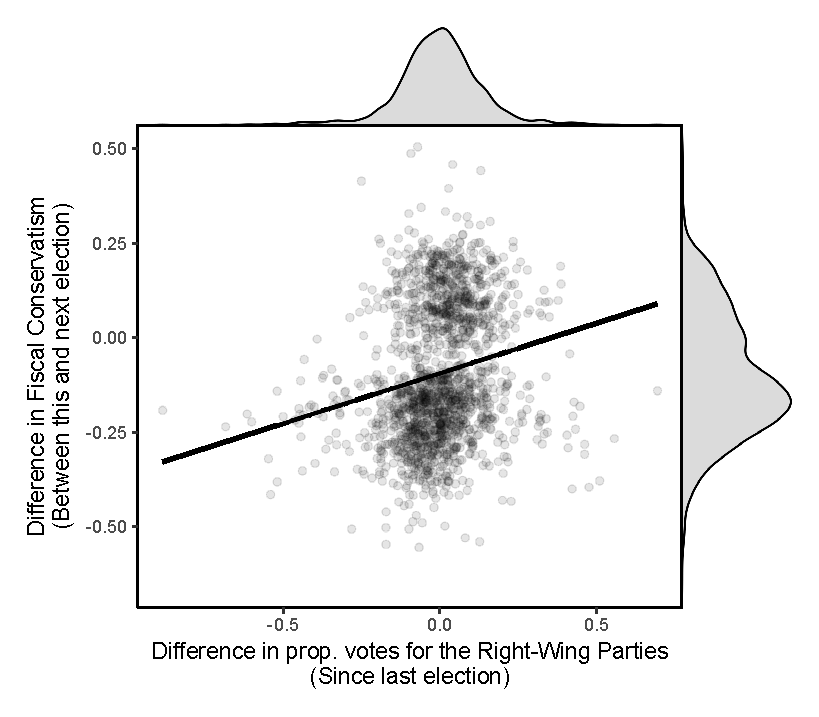
\includegraphics[scale = 1.2]{fd_plot.eps}
	\caption{....}
	\label{fig:scatter}
\end{figure}

Turning to models. 

Figure \ref{fig:FourYearLead} plots the key estimate (i.e., the effect of changes in local policy preferences; $\hat{\beta}$) from our (1) fixed effects model, (2) a pooled model which excludes time and year fixed effects, (3) a first difference model which substitutes the dependent variable for a first difference of the policy indicator and drops the unit fixed effects. The models left panel uses the full measure of fiscal conservatism as the dependent variable. Because many of the indicators have a large number of missing years, the models in the right panel includes only overall spending as well as income and property tax, as they are available throughout the entire period. Across all three models we find a statistically significant and positive effect. Furthermore, we obtain the same results using either measure of fiscal conservatism (differences in the unstandardized coefficients are driven by a larger standard deviation in the reduced measure).


In our preferred model (the fixed effects model), we estimate the effect to be 0.18 this means that if net support for right-wing parties increases with 10 percentage points, then policy becomes 0.02 more conservative. If we only look at within municipality variation in policy conservatism, then this corresponds to 10 pct. of a standard deviation.  This is a substantive association. With an effect of this magnitude, moving the voters from the socialdemocratic stronghold Albertslund to the highly conservative Gentofte would transform the fiscal policy in Gentofte to that of Slagelse. In other words, it would move Gentofte down by more than 40 positions (out of 273 municipalities) in our ranking of fiscal conservatism.

\begin{figure}[h]
	\centering
	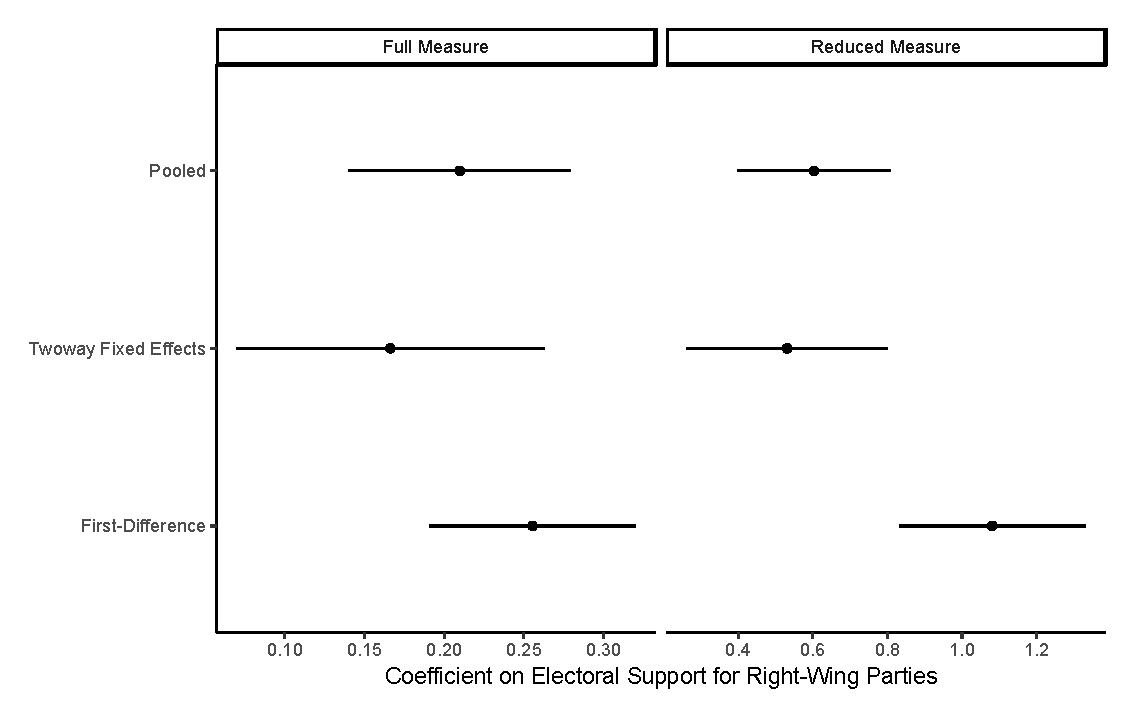
\includegraphics[scale = 0.8]{coef_31082018.eps}
	\caption{Effect of Electoral Support for Right-wing Parties with a 4-year Lead. Points are unstandardized OLS coefficients. Lines are 95 pct. confidence intervals computed using Newey-West robust standard errors.}
	\label{fig:FourYearLead}
\end{figure}


To examine the temporal dynamics of this effect, figure \ref{fig:LongRun} reports the estimated effect of local policy preferences at time $t$ on policy preferences at different points in time. In particular, it is plotted at $t=0$, one year after $t=0$, $t=1$ (corresponding to four years after $t=0$), $t=2$ (eight years), $t=3$ (16 years) and $t=4$ (20 years). This figure reveals that, as expected, it takes some time for policy to respond. There is only a small effect one year after local policy preferences change and the largest effect is  after four years. After this the effect seems to have some staying power, and while it does become smaller over time, it is remarkable that a change in voter mood can persist as far into the future as 16 years (corresponding to four elections) before disappearing.

CAN WE DO EACH YEAR ? ALSO, WE DO NOT SHOW YEAR -4.

Figure \ref{fig:LongRun} also shows that estimated effects of local policy preferences on policy conservatism at $t=0$ and $t=-4$ are statistically insignificant and close to zero. This shows that the trends in social democratic and conservative municipalities are similar prior to the electorate's mood changes. After voter preferences evolve, however, trends in policy diverge. Importantly, if voters became \emph{more conservative} as a result of changes in policy \cite[cf.][]{lenz2013follow,slothuus2010can}, and this was what was driving our result, then we would expect our estimate of pre-trend differences to be positive and statistically significant. Instead, changes in local policy preference appear to be independent of current trends in policy conservatism. This is notable, because it suggests that the key identifying assumption of our fixed effects model holds, namely, that there are parallel trends in the dependent variable (policy) before the independent variable (preferences) change.

NOTE THAT THIS IS UNIQUE. NO ONE ELSE HAVE FOUND THIS WITH CAUSAL SEPERATATION (t-1 to t+1,2,3), +LEVEL OF DETAIL.

\begin{figure}[h]
	\centering
	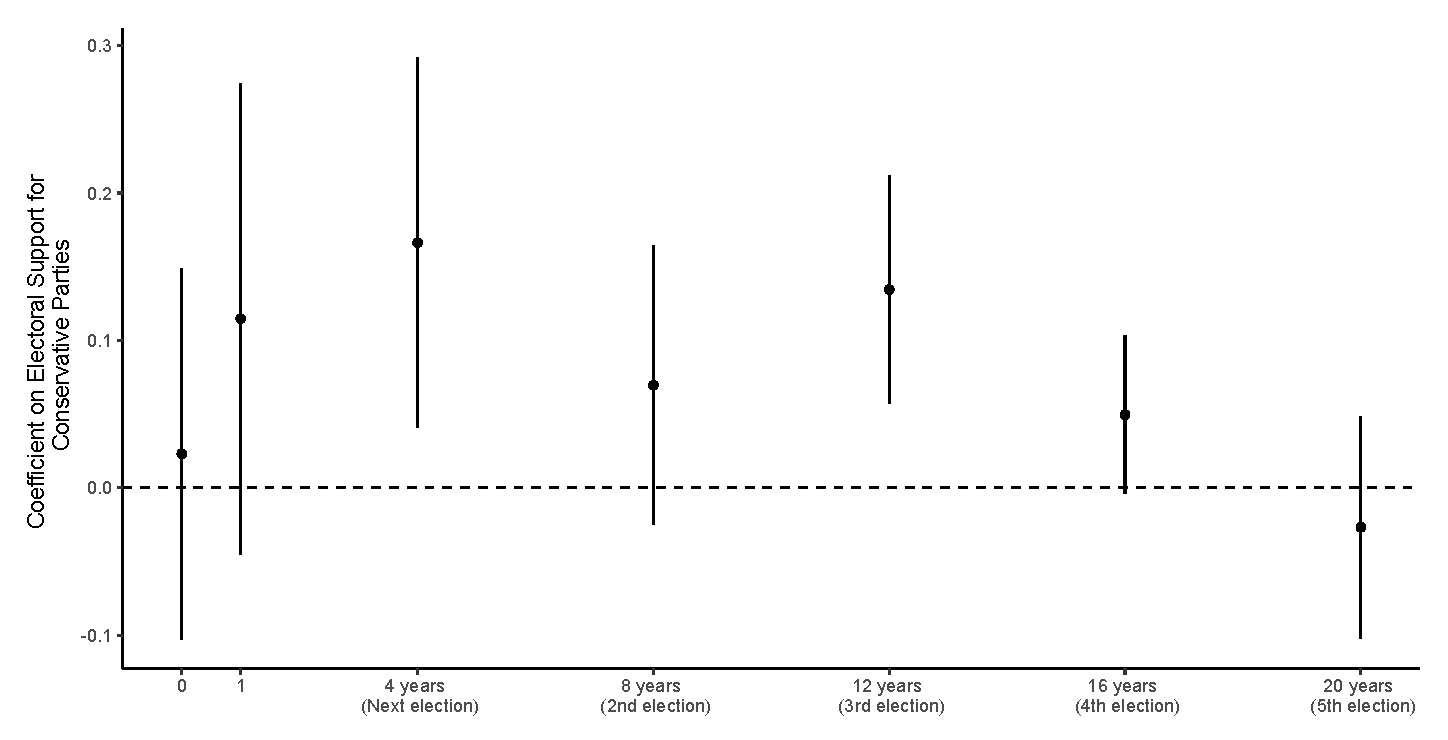
\includegraphics[scale = .6]{NoLag_varying_leads.eps}
	\caption{Effects of Local Policy Preferences Over Time. Black points represent the effect of net electoral support for conservative parties with different leads. Black lines are 95 pct. confidence intervals based on Arellano-White robust standard errors with clustering at the municipal level.}
	\label{fig:LongRun}
\end{figure}


\subsection{Evidence of Reverse Causality?}
DOES CHANGES IN POLICY AFFECT LATER CHANGES IN PREFERENCES?


\subsection{Does It Simply Reflect Fiscal Stress?}
Bad Control, Yet still relevant to look at variation independent of fiscal stress. 

\subsection{Is it Just The Mayoralty?}

There are two important reasons why we would expect municipal policy to be responsive to voter preferences. First, when the electorate chooses to elect more right-wing candidates, we would expect them to enact more fiscally conservative policies. Second, we might observe that parties are differentially responsive to voter preferences. We investigate these mechanisms in Figure \ref{fig:mech}.

In panel A, we include a categorical control for whether the mayoral party is the Liberal Party, the Social Democrats, or some third party.  In doing so, we condition the effect of electoral support for right-wing parties on, whether those parties control the most important municipal policy-making position. This gives us the effect of support for right-wing parties among the voters after taking into account, which politicians they elect. Identifying the direct effect of electoral support net of selection by including a post-treatment control in this way requires very strong assumptions that are unlikely to be met \textbf{REFERENCE}. Still, it is striking how little the coefficient on the policy preferences of the electorate changes, when controlling for the mayoral party. This result is very similar to 

\begin{figure}
	\begin{subfigure}{0.45\textwidth}
		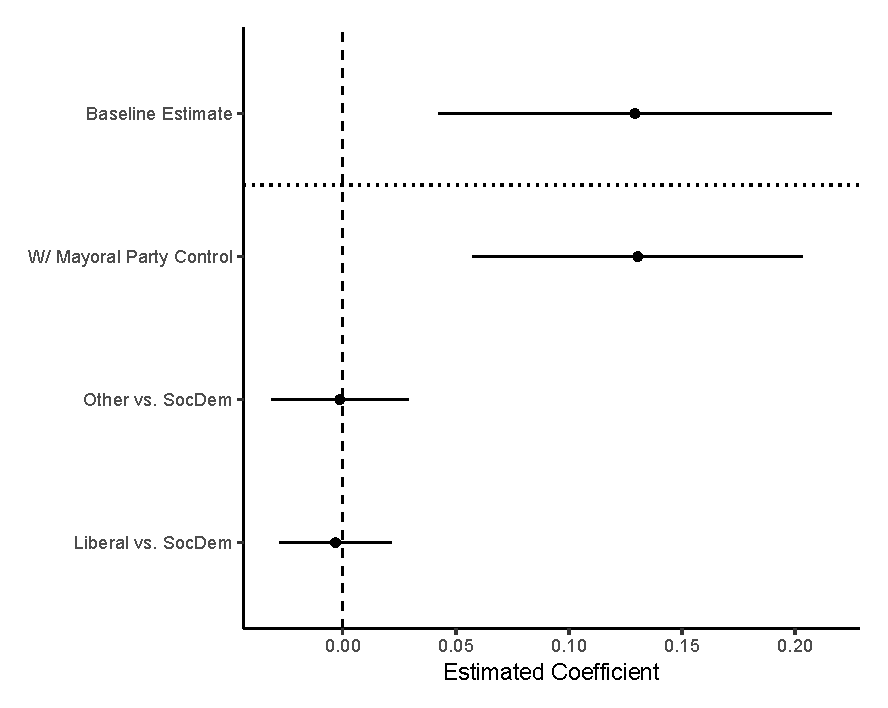
\includegraphics[width=1\textwidth]{PostTreatControl.eps}
		\caption{Are Results Driven by Selection? The figure shows results after including control for the mayoral party. Baseline estimates are included for comparison.} \label{mech}
	\end{subfigure}  \hfill
	\begin{subfigure}{0.45\textwidth}
		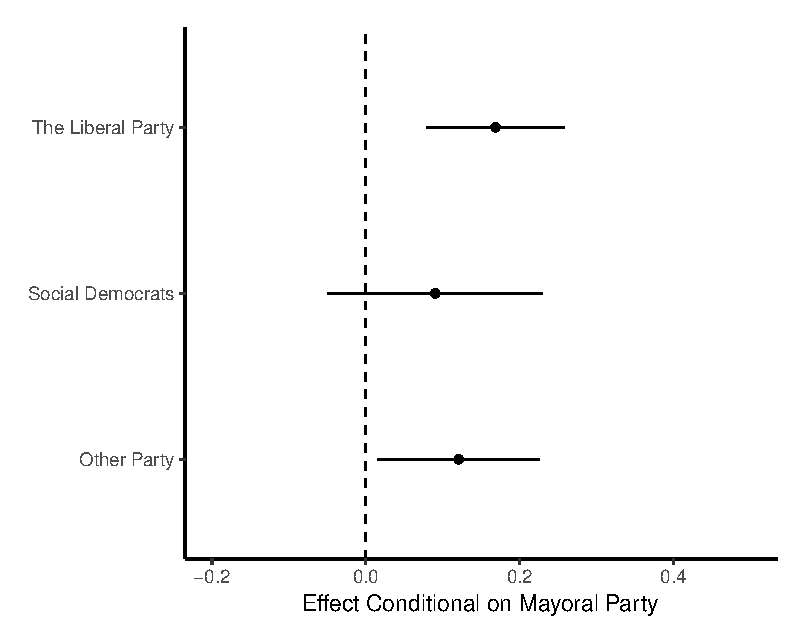
\includegraphics[width=1\textwidth]{MargFX_31082018.eps}
		\caption{Are All Parties Equally Responsive? The figure shows the marginal effects from a model including an interaction between mayoral party and electoral support for right-wing parties.} \label{inter}
	\end{subfigure}
	\caption{Responsiveness or Selection? Twoway fixed effects and population size (logged) included in both models. Confidence intervals are 95 pct., computed from Newey-West robust standard errors.}
	\label{fig:mech}
\end{figure}

In panel B, we allow the effect to vary across our three different categories of mayoral party. While there is too much noise in the estimation for the differences to be statistically significant, the point estimates for the two major parties (Social Democratis and the Liberal Party) are strikingly similar. Both estimates are large, and we can reject the null at a reasonably high level of confidence. For third-party mayors, however, we cannot reject the null that they are unresponsive to voter preferences.


\section{Discussion \& Conclusion}
We find a solid effect. In line with recent studies that take measurement seriously. 

Replication in other contexts

\bibliographystyle{apa}
\bibliography{bibtex/library}

\clearpage

\renewcommand{\thesubsection}{\Alph{subsection}}
\renewcommand{\thetable}{\Alph{subsection}\arabic{table}}
\renewcommand{\thefigure}{\Alph{subsection}\arabic{figure}}

\section*{Appendix: For Online Publication}

\localtableofcontents

\clearpage
\subsection{Overview of Policies Included in Our Measure}

\begin{table}[h]
	\centering \footnotesize
	%\caption{Indicators of Fiscal Policy Conservatism}
	\label{tab:policies} 
	\begin{tabular}{p{5.5cm}P{3cm}P{4.5cm}} \hline
		\textbf{Policy}                          & \textbf{Availabiliy \newline (number of years)} & \textbf{Do Higher or Lower Values Imply Conservatism?} \\
		\hline
		&&\\ \textit{Tax policy} &&\\
		Income tax (pct.)                        & 29     &    Lower       \\
		Property tax (per mille)                      & 29    &    Lower        \\
		Commercial real estate tax (per mille) & 14    &    Lower               \\ \hline
	
		&&\\ \textit{Spending policy}  &&\\
		Spending pr. capita (DKK)                & 29    &    Lower        \\
		Spending pr. pupil in school (DKK)       & 7     &    Lower     \\ \hline
		
		&&\\\textit{Organization of public service delivery}  &&\\
 		Public Employees (pr. 1,000 citizens)	 & 9	  &	   Lower	     \\
 		Privately operated services  (pct.) &   14  &    Higher     \\
 		Purchases with a private supplier  (pct.)      & 14    &    Higher     \\ \hline
 	
 		&&\\ \textit{Co-payment for public services} &&\\   
		Average cost of day care (DKK)                  & 16    &    Higher     \\
		Price of relief stay (DKK)				 & 7	  &	   Higher	 \\
		Food delivery for the  elderly (DKK) & 7   &    Higher     \\
		Stay in nursing home (DKK)              & 7     &    Higher     \\ \hline
	
		&&\\ \textit{Extent of Public Services} &&\\ 
		Public housing (pct.)                    & 14     &    Lower               \\
		Class size in public schools	         & 14    &    Lower       \\
		\hline \hline
		\end{tabular}
\end{table} 

\clearpage

\subsection{Details about Estimation}

\clearpage

\subsection{Some Descriptive Features of Municipal Fiscal Policy}

Figure \ref{fig:descriptive} presents some descriptive features of the annual measure of fiscal policy conservatism. In particular, it looks at how the measure is distributed across time and space, revealing some interesting patterns in municipal fiscal policy.

Fiscal policy conservatism dropped slightly in the period. The drops are located in '78 to 81 and from 93 to 2000: periods where the Social Democratic Party was in power nationally. This makes sense as liberal national fiscal policies are likely to spill over into local politics through intergovernmental grants etc.

Aside from the national trends, however, the most notable feature of the time series seems to be the large variation we identify in fiscal policy. Some municipalities are, apparently, very fiscally conservative while others are very liberal. Although the within-differences are less dramatic, we also see some municipalities start out more conservative and then become more liberal and vice versa.

Further, the geographic spread of fiscal conservatism matches what most observers of Danish politics would expect. The most conservative municipalities are in Western Jutland and North of Copenhagen whereas the most Liberal (or Socialist) municipalities are west of Copenhagen and in an around the other large cities (Aaalborg, Aarhus, Odense). 
Figure \ref{mostleast} presents an overview of the most and the least conservative municipalities across the entire period.





\begin{sidewaysfigure}[htbp]
	\centering 
	\begin{subfigure}[h]{0.38\textwidth} 
		\includegraphics[width=1\textwidth]{newtimes_lines.eps}
		\caption{Average Municipal Fiscal Policy Conservatism (dark line) and Municipal Fiscal Policy Conservatism for Individual Municipalities (grey lines) from 1978 to 2006.}
		\label{fig:timeline}
	\end{subfigure} \hspace{1cm}
	\begin{subfigure}{0.38\textwidth} 
		\includegraphics[width=1\textwidth]{newJoyPlotFiscal.eps}
		\caption{Distribution of Municipal Fiscal Policy Conservatism from 1978 to 2006 (densities).}
		\label{fig:lines}
	\end{subfigure}
	\begin{subfigure}{0.9\textwidth} 
		\includegraphics[width=1\textwidth]{Map_of_FiscCon.eps}
		\caption{The Geographic Distribution of Municipal Fiscal Policy Conservatism at Three Points in Time.}
		\label{fig:map}
	\end{subfigure} 
	
	\caption{How has Municipal Fiscal Policy Conservatism Developed from 1978 to 2006?}
	\label{fig:descriptive}
	
\end{sidewaysfigure}

\begin{figure}
	\centering
	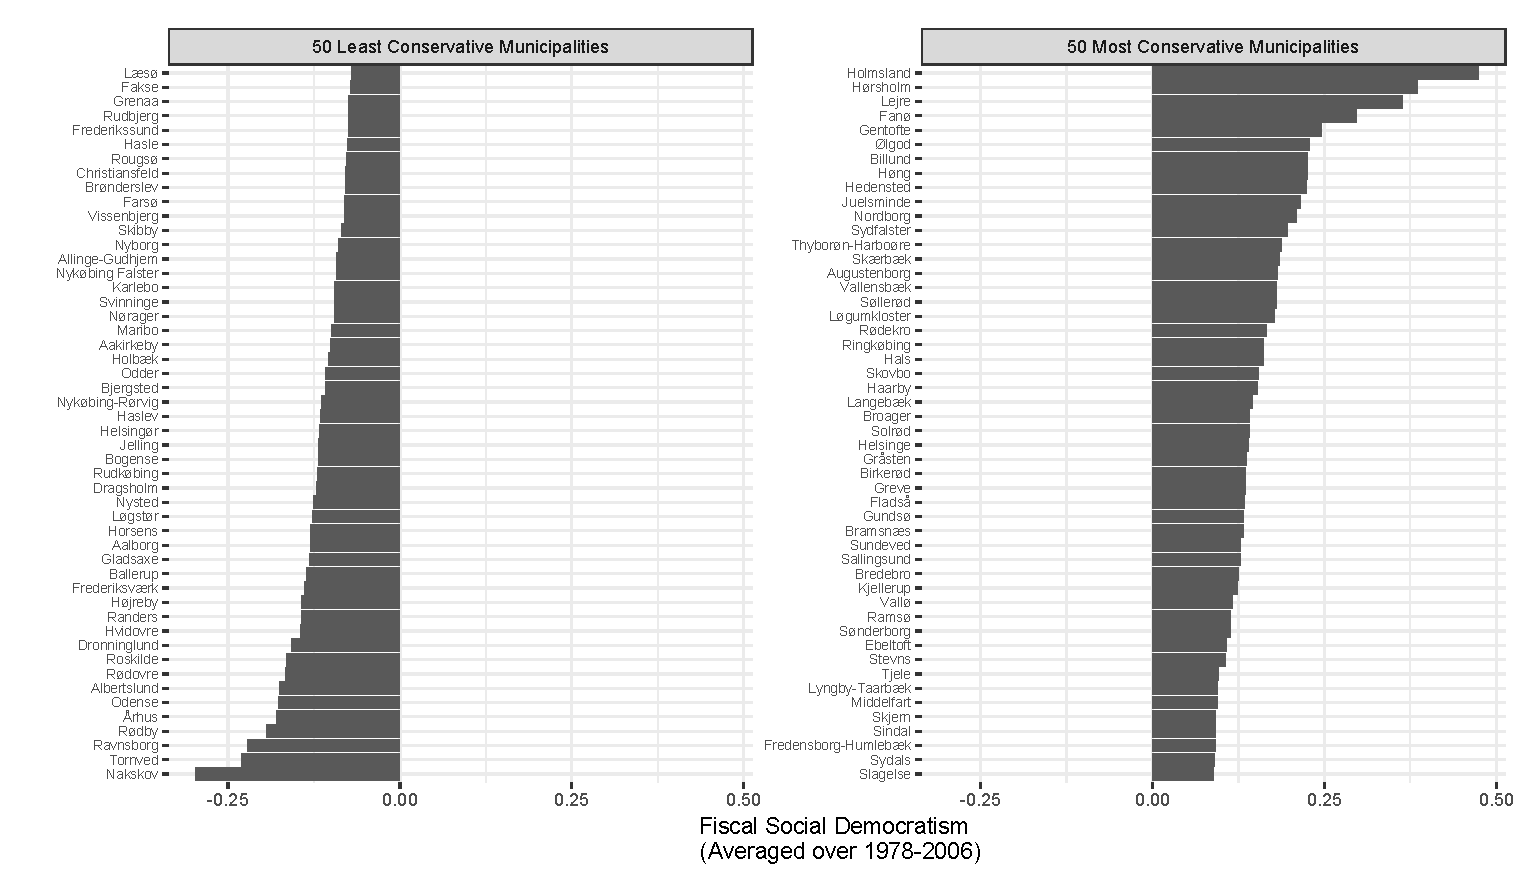
\includegraphics[width=1\textwidth]{socialdemocratism.eps}
	\caption{The Most and Least Conservative Municipalities} \label{mostleast}
\end{figure}

\clearpage

\subsection{Some More Context On Danish Municipalities}
There have been two large reforms of local politics in the last 50 years. The first was conducted in 1970 as the Danish welfare state started to expand. Here the number of municipalities were reduced from more than 1000 to 275 \citep{ingvartsen1991kommunalreformen}. (Although it was 277 the first two years.)  The second reform was conducted in 2007 and further reduced the number of municipalities from 275 to 98. Once again, the increasing complexity of public service provision was a key argument for the reform \citep{christiansen2008utaenkelige}. Since both of these reforms were comprehensive in terms of amalgamations and changes to the relative power of national ctr. local government, we let them be the bookends of our analysis, examining the relationship between citizens policy views and the ideological flavor of municipal policy between the two reforms.\footnote{In this study, we exclude the municipality of Copenhagen and Frederiksberg, as these were governed in a different way.} Because of data availability we further limit our study period, so that it goes from 1978 and 2008.

In the period we study, Danish municipalities are governed by small city councils (between 9 and 29 members) which are elected at proportional elections and with a multi-party system which, to a large extent, mirrors the party system at the national level \citep{blom2013et}. Elections are fixed to take place every four years and do not usually coincide with elections at the national or EU level.\footnote{There was only three years between the elections of 1981 and 1978} Turnout is high with an average of around 70 percent since 1970.  

Following each municipal election, a majority in the city council elects a mayor, and the chairmen of the various committees \citep{serritzlew2008explaining}. Mayors are the only full time professional politicians in the city councils and have a number of formal obligations \citep{kjaer2015urban}. Mayors are also responsible for the day-to-day business of the administration and chairs the important economic committee which sets taxes and the budget. The work in the city council is structured by a a number of committees. The number and size of the committees is determined by the council. Committee membership is allocated proportionality between the political parties which means that there is broad political representation in all committees. The committees can decide on matters in their area and the administrative responsibility across areas is therefore essentially divided. 


\subsection{Validating Our Measure Of Citizens' Policy Preferences}
How well does this electoral measure capture voters underlying preferences? To get an indication of this, we look at the 2013 Danish Municipal Election Survey \cite{elklit2017kv13}. In this survey, more than 30 respondents (avg. 46) from each municipality were asked to place themselves on an eleven point ideology scale going from left to right. We calculate the municipality-specific mean of these responses and correlate these with the municipality-specific net support for conservative parties in the 2013 municipal election.  As can be seen from figure \ref{validation1}, the two are strongly correlated, which suggests that we are in fact tapping into relevant variation in policy views, when we measure citizens preferences over parties. Further, its important to note that the correlation is biased downwards, because we have random measurement error in our sample based measure of policy views.\footnote{The reader should also note that due to the municipal reform of 2006 (cf. the section on empirical context) we can only have 98 observations corresponding to the 98 (amalgamated) municipalities.}

\begin{figure}[htbp]
	\begin{subfigure}{0.45\textwidth}
		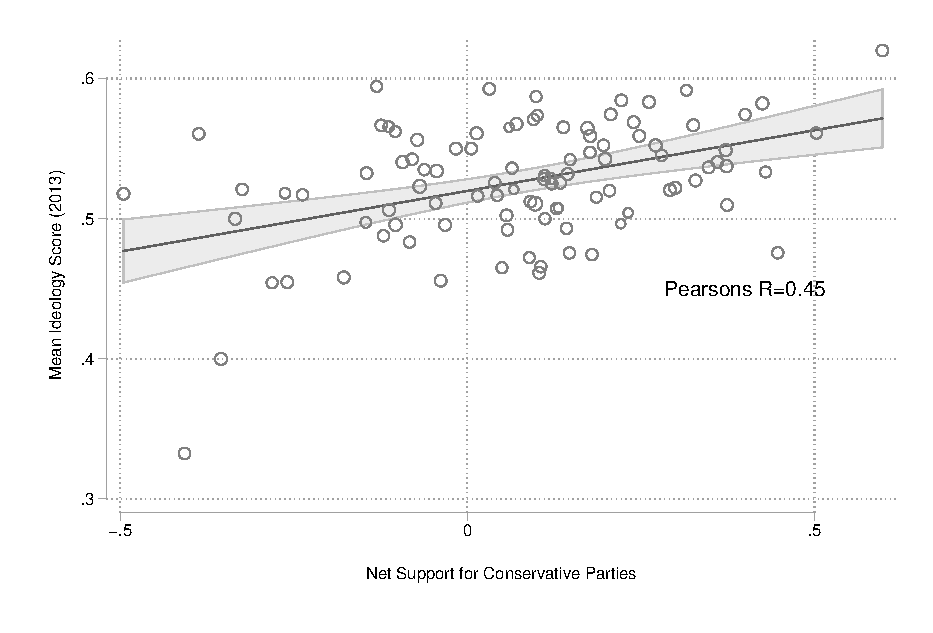
\includegraphics[width=1\textwidth]{validation.eps}
		\caption{Does the electorates preference over parties reflect preferences over policy? Data from the 2013 municipal election.} \label{validation1}
	\end{subfigure}  \hfill
	\begin{subfigure}{0.45\textwidth}
		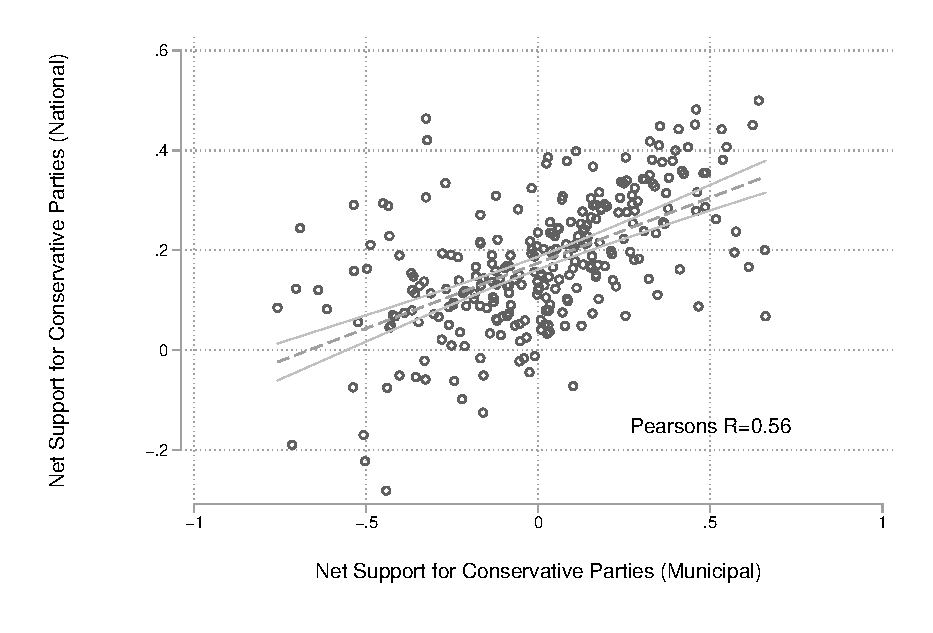
\includegraphics[width=1\textwidth]{validation2.eps}
		\caption{How strongly correlated are the electorate's preferences at municipal and national elections? Data from the 2005 municipal and national elections.} \label{validation2}
	\end{subfigure}
	\caption{How does our measure of local policy preferences perform?}
\end{figure}

Our measure of local policy preferences do not simply reflect the overall ideological mood in the municipality, but the ideological mood expressed by the electorate at municipal elections. This is potentially significant, because unlike previous research, which relies on electoral data from national or regional elections, we do not risk misidentifying electorates who might differ in their policy views across domains (i.e., who want more liberal fiscal policies locally and more conservative policies nationally). Why might there be a divergence between the electorate's preferences at a local and at a national election? For one, the electorate at municipal elections might be differently composed than electorates in national elections, as different types of people participate in different types of elections \citep{ansolabehere2015beyond,hansen2017social} In addition to this, voters might have preferences over which levels of government should be smaller or larger.

In figure \ref{validation2}, we try to gauge the extent to which it matters that our measure relies on data from municipal rather than national elections. To do this, we correlate  municipal-level net support for conservative parties at the 2005 municipal election with municipal-level net support for the same conservative parties at a national election held six months earlier. This analysis reveals a strong, but in no way deterministic, correlation of 0.56. Accordingly, we might miss meaningful variation, if we used election returns from national, rather than local, elections to estimate local policy preferences.

\clearpage

\subsection{An Alternative Measure of City Policy Preferences}

\clearpage

\subsection{Effects on Individual Policy Indicators}

\clearpage

\subsection{Models With Controls}

\clearpage

\end{document}